\documentclass[border=2mm]{standalone}
\usepackage{tikz}
\usetikzlibrary{positioning,shapes.geometric,arrows.meta}

% Define academic-friendly colors
\definecolor{vocabcolor}{RGB}{25,118,210}
\definecolor{practicecolor}{RGB}{245,124,0}
\definecolor{testcolor}{RGB}{76,175,80}
\definecolor{operatecolor}{RGB}{255,193,7}

\begin{document}
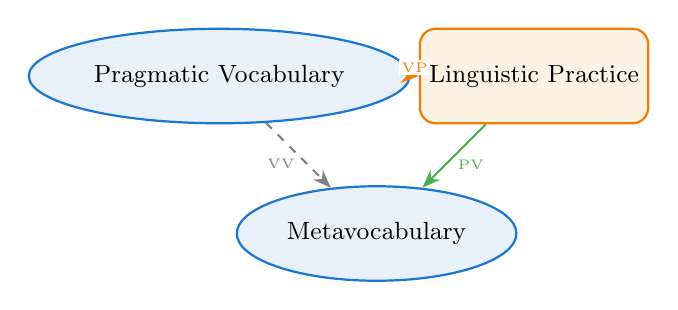
\begin{tikzpicture}[>=Stealth]
  % Node styles for academic quality
  \tikzset{
    vocabulary/.style={ellipse, draw=vocabcolor, fill=vocabcolor!10, thick, minimum width=2.5cm, minimum height=1.2cm, text centered, font=\small},
    practice/.style={rectangle, draw=practicecolor, fill=practicecolor!10, thick, minimum width=2.5cm, minimum height=1.2cm, rounded corners=2mm, text centered, font=\small},
    test/.style={diamond, draw=testcolor, fill=testcolor!10, thick, minimum width=2cm, minimum height=2cm, text centered, font=\small},
    operate/.style={rectangle, draw=operatecolor, fill=operatecolor!10, thick, minimum width=2.5cm, minimum height=1.2cm, text centered, font=\small},
    pv/.style={->, thick, color=testcolor},
    vp/.style={->, thick, color=practicecolor},
    pp/.style={->, thick, color=purple},
    vv/.style={->, thick, color=red},
    resultant/.style={->, thick, dashed, color=gray}
  }

  % Example nodes (this would be generated by the tool)
  \node[vocabulary] (vocab1) at (0, 2) {Pragmatic Vocabulary};
  \node[practice] (practice1) at (4, 2) {Linguistic Practice};
  \node[vocabulary] (vocab2) at (2, 0) {Metavocabulary};
  
  % Example edges (this would be generated by the tool)
  \draw[vp] (vocab1) -- (practice1) node[midway, above, font=\tiny, fill=white, inner sep=1pt] {VP};
  \draw[pv] (practice1) -- (vocab2) node[midway, below right, font=\tiny, fill=white, inner sep=1pt] {PV};
  \draw[resultant] (vocab1) -- (vocab2) node[midway, below left, font=\tiny, fill=white, inner sep=1pt] {VV};
\end{tikzpicture}
\end{document}